\documentclass[11pt]{article}
\usepackage[utf8]{inputenc}	% Para caracteres en español
\usepackage{amsmath,amsthm,amsfonts,amssymb,amscd}
\usepackage{multirow,booktabs}
\usepackage[table]{xcolor}
\usepackage{fullpage}
\usepackage{lastpage}
\usepackage{enumitem}
\usepackage{fancyhdr}
\usepackage{mathrsfs}
\usepackage{wrapfig}
\usepackage{setspace}
\usepackage{calc}
\usepackage{multicol}
\usepackage{cancel}
\usepackage[retainorgcmds]{IEEEtrantools}
\usepackage[margin=1cm]{geometry}
\usepackage{amsmath}
\newlength{\tabcont}
\setlength{\parindent}{0.0in}
\setlength{\parskip}{0.05in}
\usepackage{empheq}
\usepackage{framed}
\usepackage[most]{tcolorbox}
\usepackage{xcolor}
\usepackage{graphicx}
\usepackage{listings}
% -- Basic formatting
\usepackage[utf8]{inputenc}
\usepackage[english]{babel}
\usepackage{times}
\usepackage{caption}
\usepackage{subcaption}
\usepackage{placeins}
\setlength{\parindent}{0pt}
\usepackage{indentfirst}% -- Defining colors:
\usepackage[dvipsnames]{xcolor}
\definecolor{codegreen}{rgb}{0,0.6,0}
\definecolor{codegray}{rgb}{0.5,0.5,0.5}
\definecolor{codepurple}{rgb}{0.58,0,0.82}
\definecolor{backcolour}{rgb}{0.95,0.95,0.92}% Definig a custom style:
\lstdefinestyle{mystyle}{
    backgroundcolor=\color{backcolour},   
    commentstyle=\color{codepurple},
    keywordstyle=\color{NavyBlue},
    numberstyle=\tiny\color{codegray},
    stringstyle=\color{codepurple},
    basicstyle=\ttfamily\footnotesize\bfseries,
    breakatwhitespace=false,         
    breaklines=true,                 
    captionpos=t,                    
    keepspaces=true,                 
    numbers=left,                    
    numbersep=5pt,                  
    showspaces=false,                
    showstringspaces=false,
    showtabs=false,                  
    tabsize=2
}% -- Setting up the custom style:
\lstset{style=mystyle}
\lstset{
  style=mystyle,
  framexleftmargin=3.5mm,
  rulesepcolor=\color{black},
  linewidth=0.6\linewidth,
  xleftmargin=12pt,
  aboveskip=12pt,
  belowskip=12pt
}
\colorlet{shadecolor}{orange!15}
\parindent 0in
\parskip 1pt
\geometry{margin=1in, headsep=0.25in}
\theoremstyle{definition}
\newtheorem{defn}{Definition}
\newtheorem{reg}{Rule}
\newtheorem{exer}{Exercise}
\newtheorem{note}{Note}
\graphicspath{ {./images/} }
\begin{document}
\setcounter{section}{0}
\title{MIE223 Lecture Notes}

\thispagestyle{empty}

\begin{center}
{\LARGE \bf Social Network Data Analysis}\\
{\large MIE223}\\
Winter 2025
\end{center}
\section{Social Network Analysis}
\subsection{Networks: An organization - HP Labs}
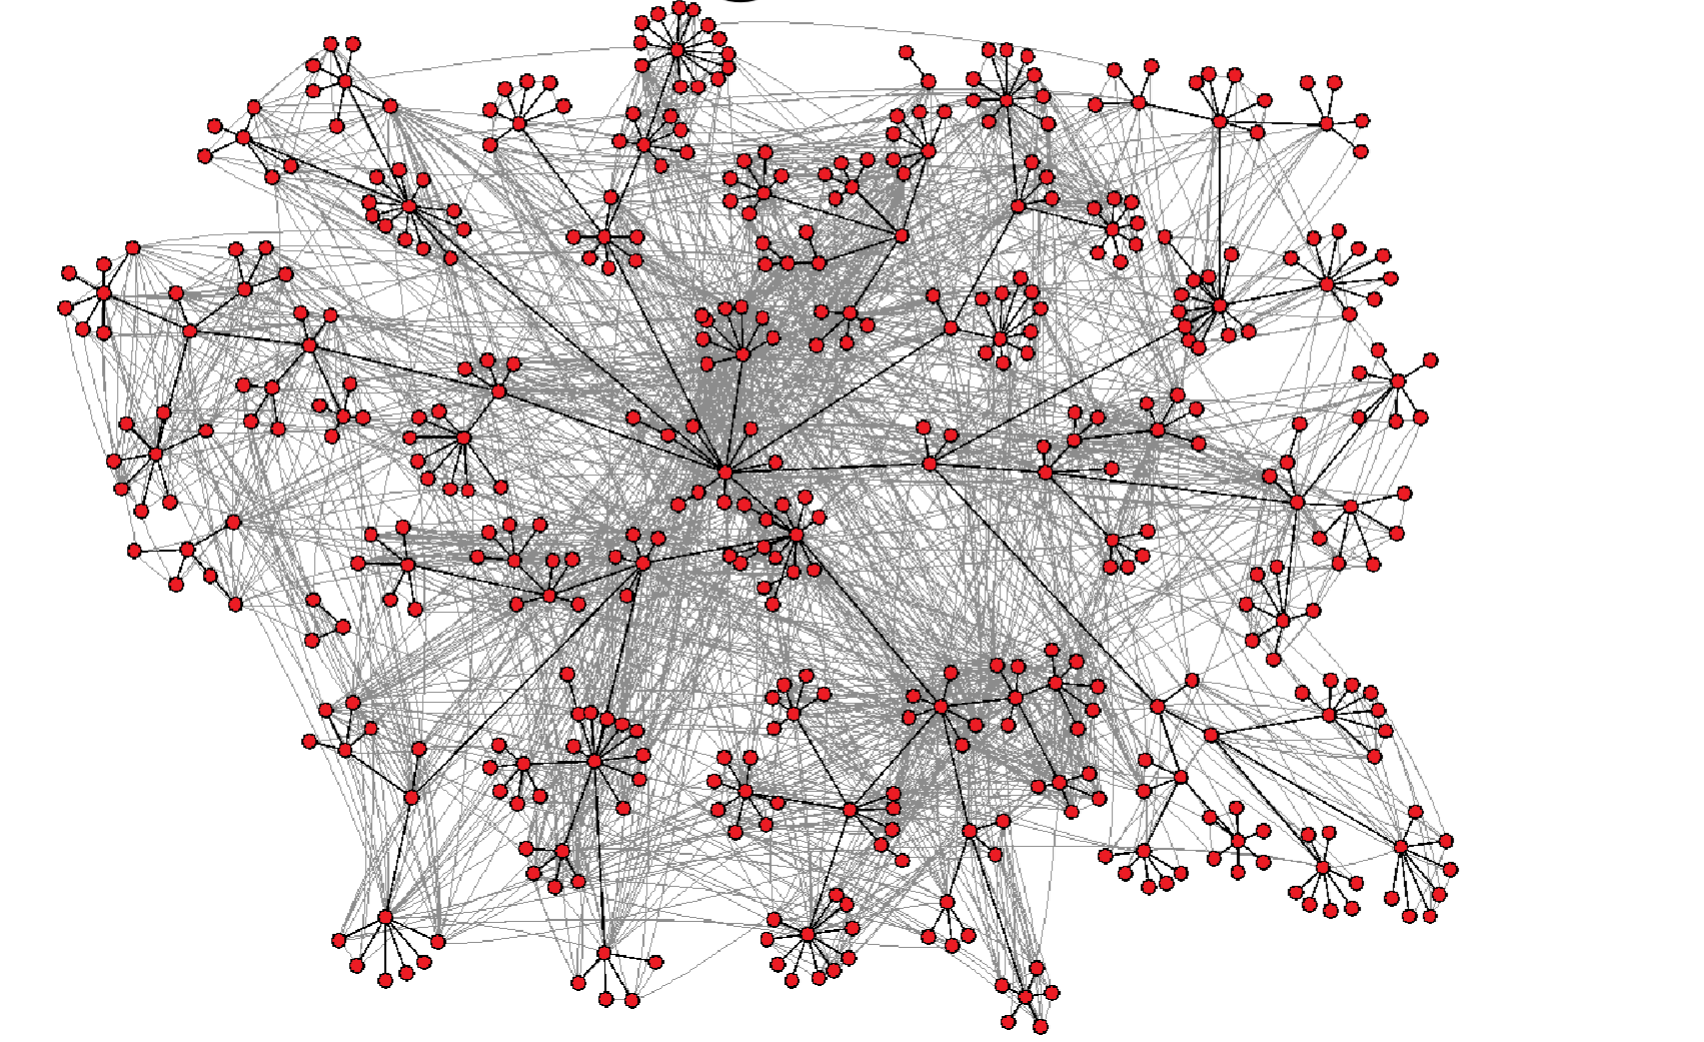
\includegraphics[width=\textwidth/2]{1.png}

not a lot of inter-team communication as they are present together.
the network represents the email communication between the teams.
holistic interconnectivity exists where the center dot is.
there is a clear tree hierarchy, with clumpiness where certain nodes
have high degree connections. social networks are not random, they are
structured.

\subsection{Political blogs}
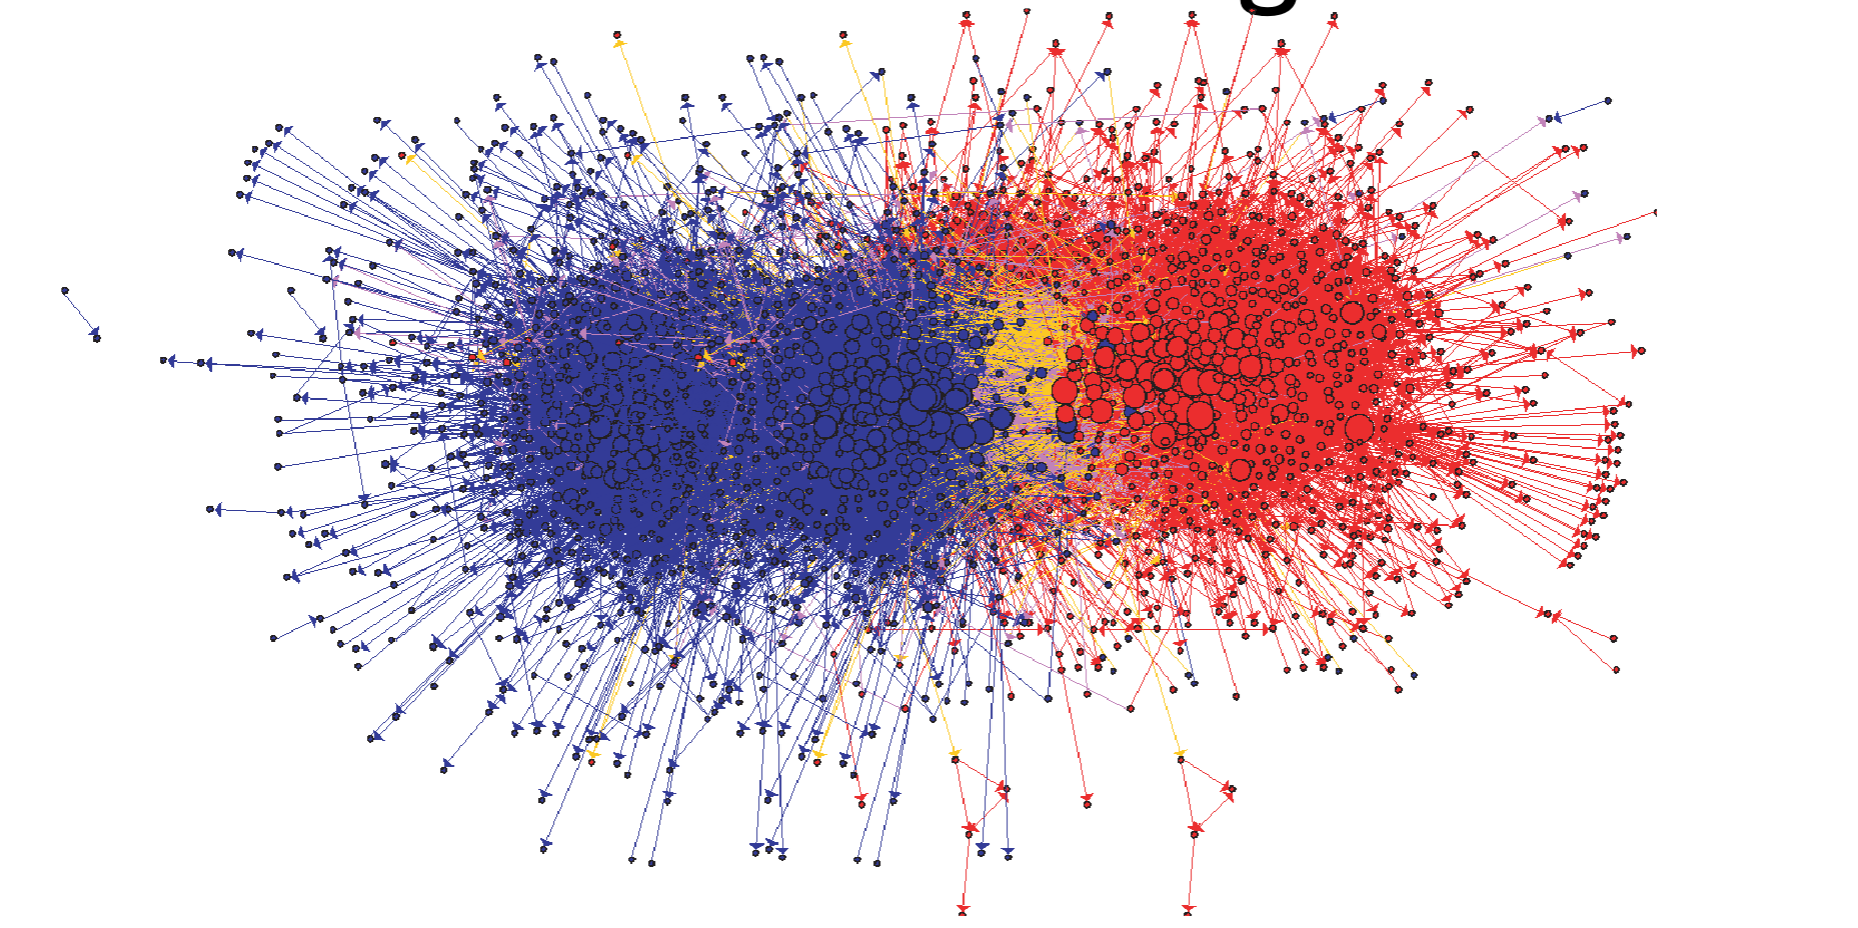
\includegraphics[width=\textwidth/2]{2.png}

the network represents the links between political blogs.
the network is divided into two main groups, with a few blogs
connecting the two groups. there are a lot of echo chambers.
\subsection{A View of Facebook via 10 M links}
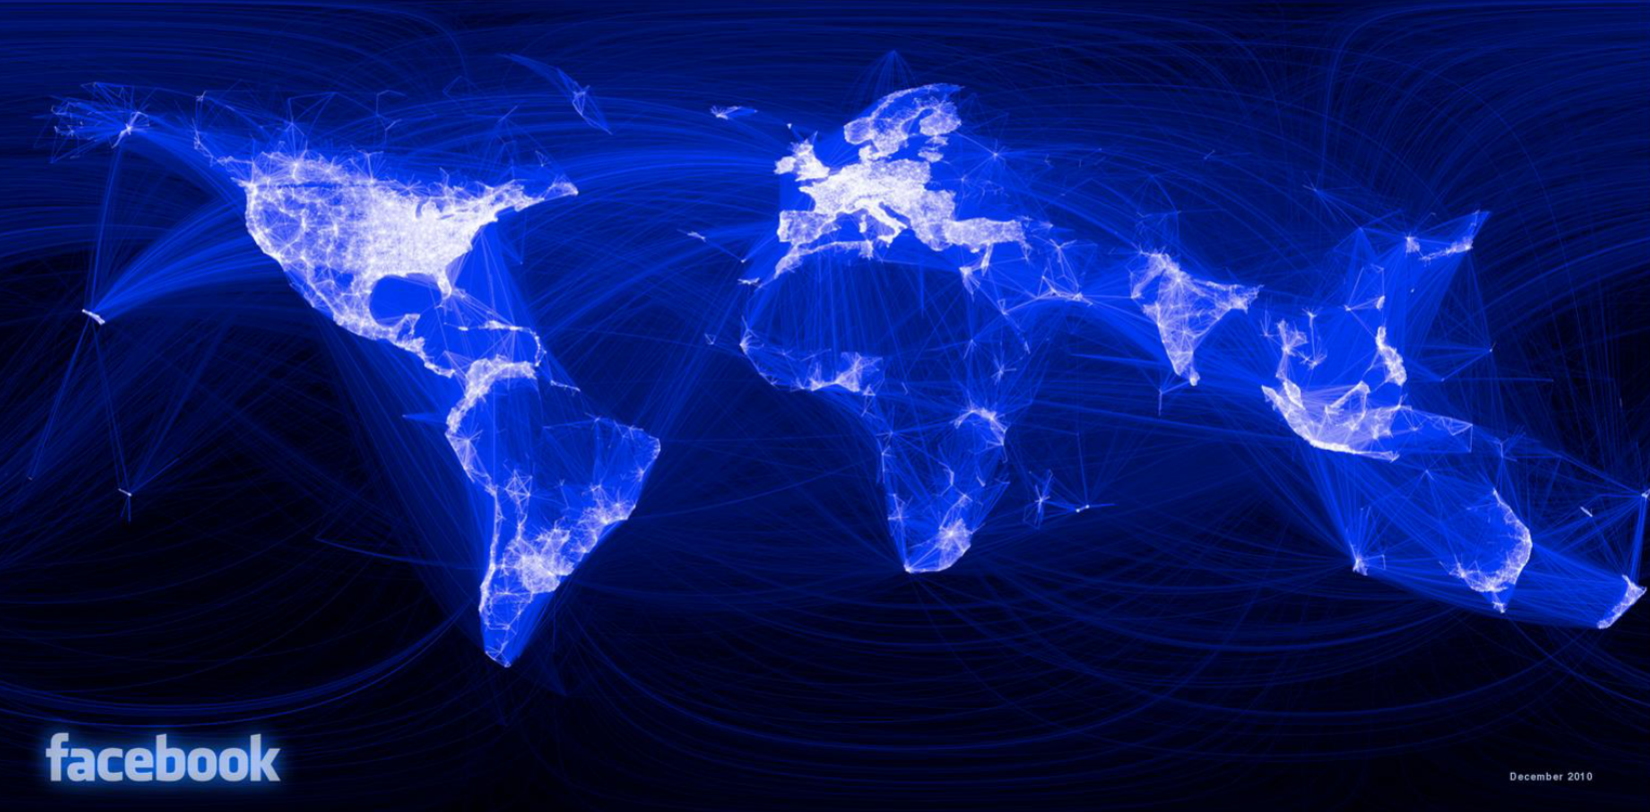
\includegraphics[width=\textwidth/2]{3.png}

data is generated by a process, which is subject to selection biases.

\subsection{Why Networks?}
Behind each of these complex systems there
is an intricate wiring diagram, a network that
defines the interactions between system
components.

Understanding the network is key to understand
the behaviors of such complex system.

\subsection{Networks}
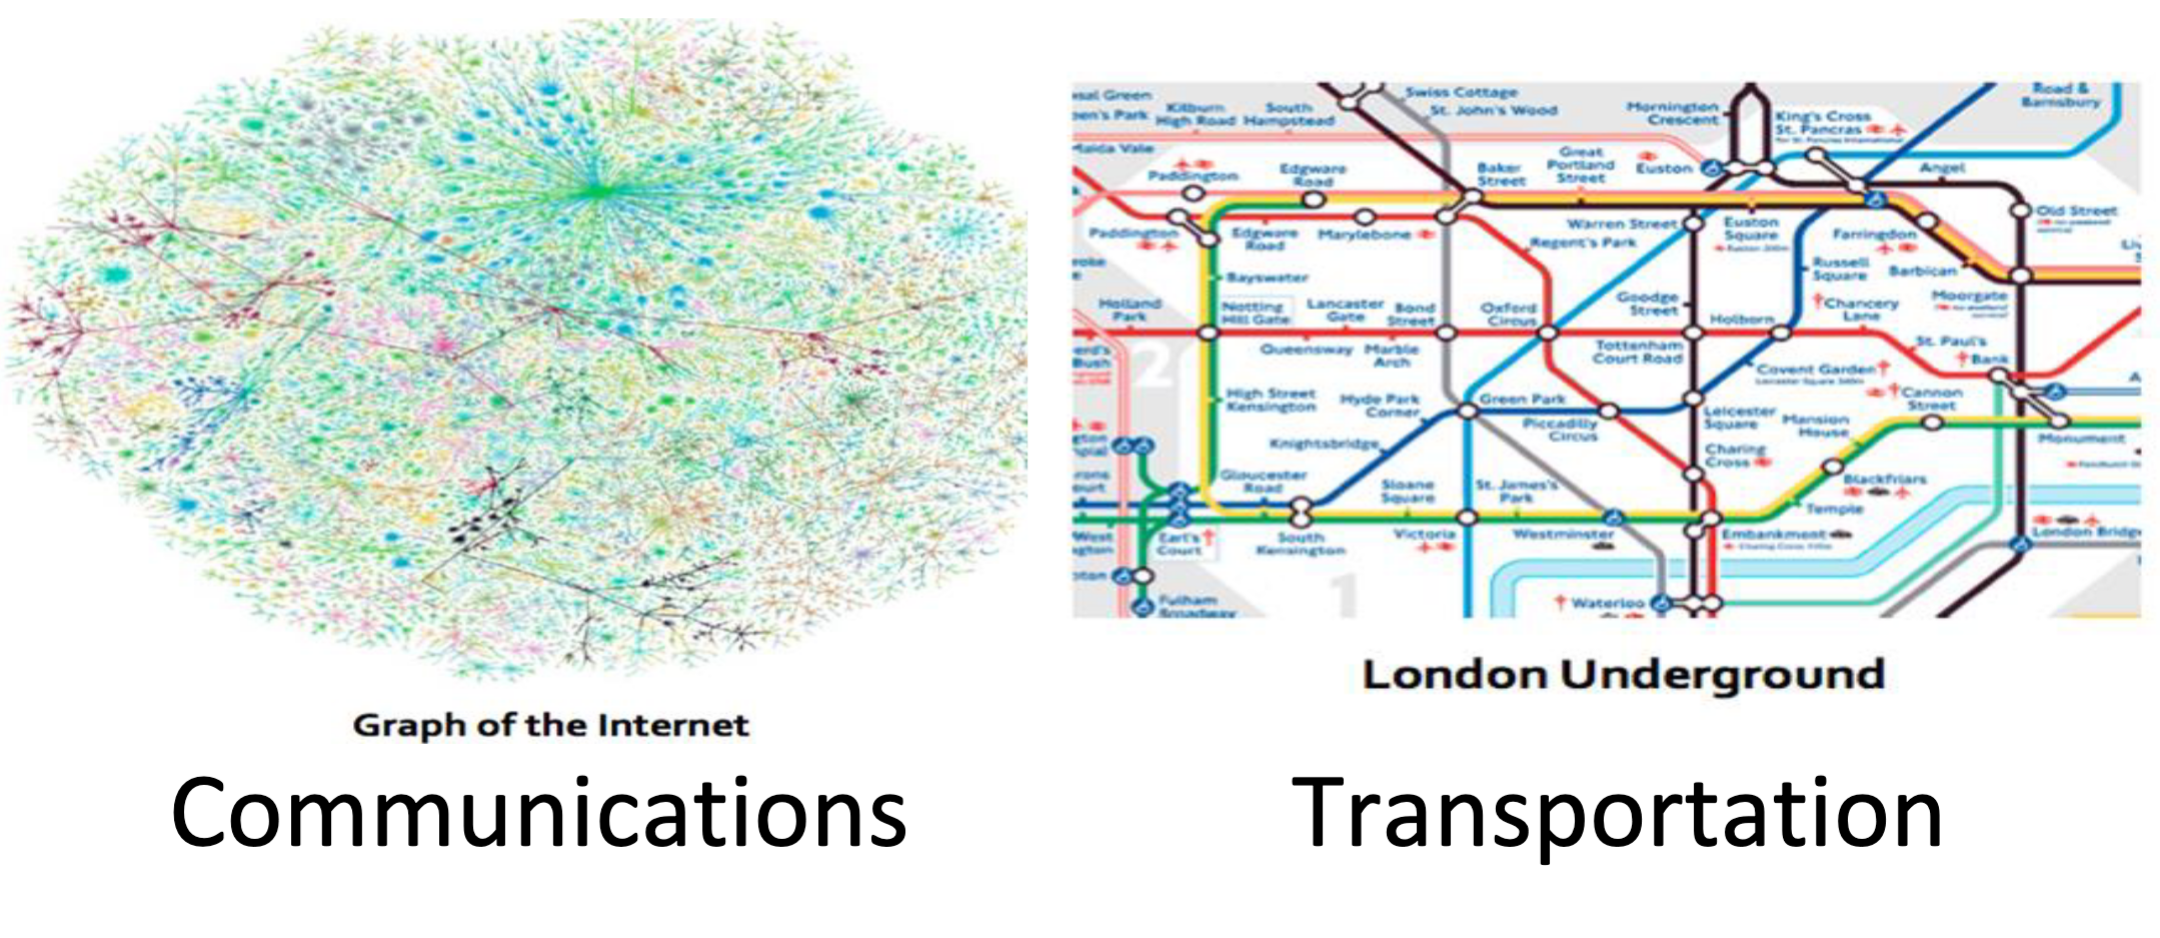
\includegraphics[width=\textwidth/2]{4.png}

\subsection{Application domains in network analysis}
\begin{itemize}
    \item Social (people-people) networks (social network)
    \item Information networks (social network)
    \item Organization and political networks (social network)
    \item Computer networking
    \item Biology
    \item Transportation networks
\end{itemize}

\section{EXAMPLES OF PROBLEMS IN
SOCIAL NETWORKS}
\subsection{E.g. 1: Small-world phenomena}
how do you decide which nodes connect to what in a social network?
there is a tree pattern in the connections, where there are supernodes with multiple connections
and other nodes where they only have a few connections.
you are more likely to friend a node if that node already has a lot of friends.

everyone is at most 60 degrees of connection away from each other

there is a power law connection in how nodes with many connections tend to gain more 
connections. these have a natural hierarchal structure and are not random.
\subsection{E.g. 1 (cont.): Link prediction}
“Given a snapshot of a social network, can we infer which new interactions
among its members are likely to occur in the near future?"
\begin{itemize}
    \item What are the measurements?
    \item -- “proximity” and “similarity” between two unconnected nodes
    \item What are application domains?
    \item -- social networks, friend recommendation; product / webpage
    recommendation; predicting academic collaborations; predicting merger and
    acquisitions ...
    \item How to measure performance?
    \item -- use future held-out data, conversion rate, ..
\end{itemize}

there is a connectivity such that you are more likely to connect to 
people your friends are connected to

\subsection{E.g. 2: Tracking Memes – What goes Viral?}
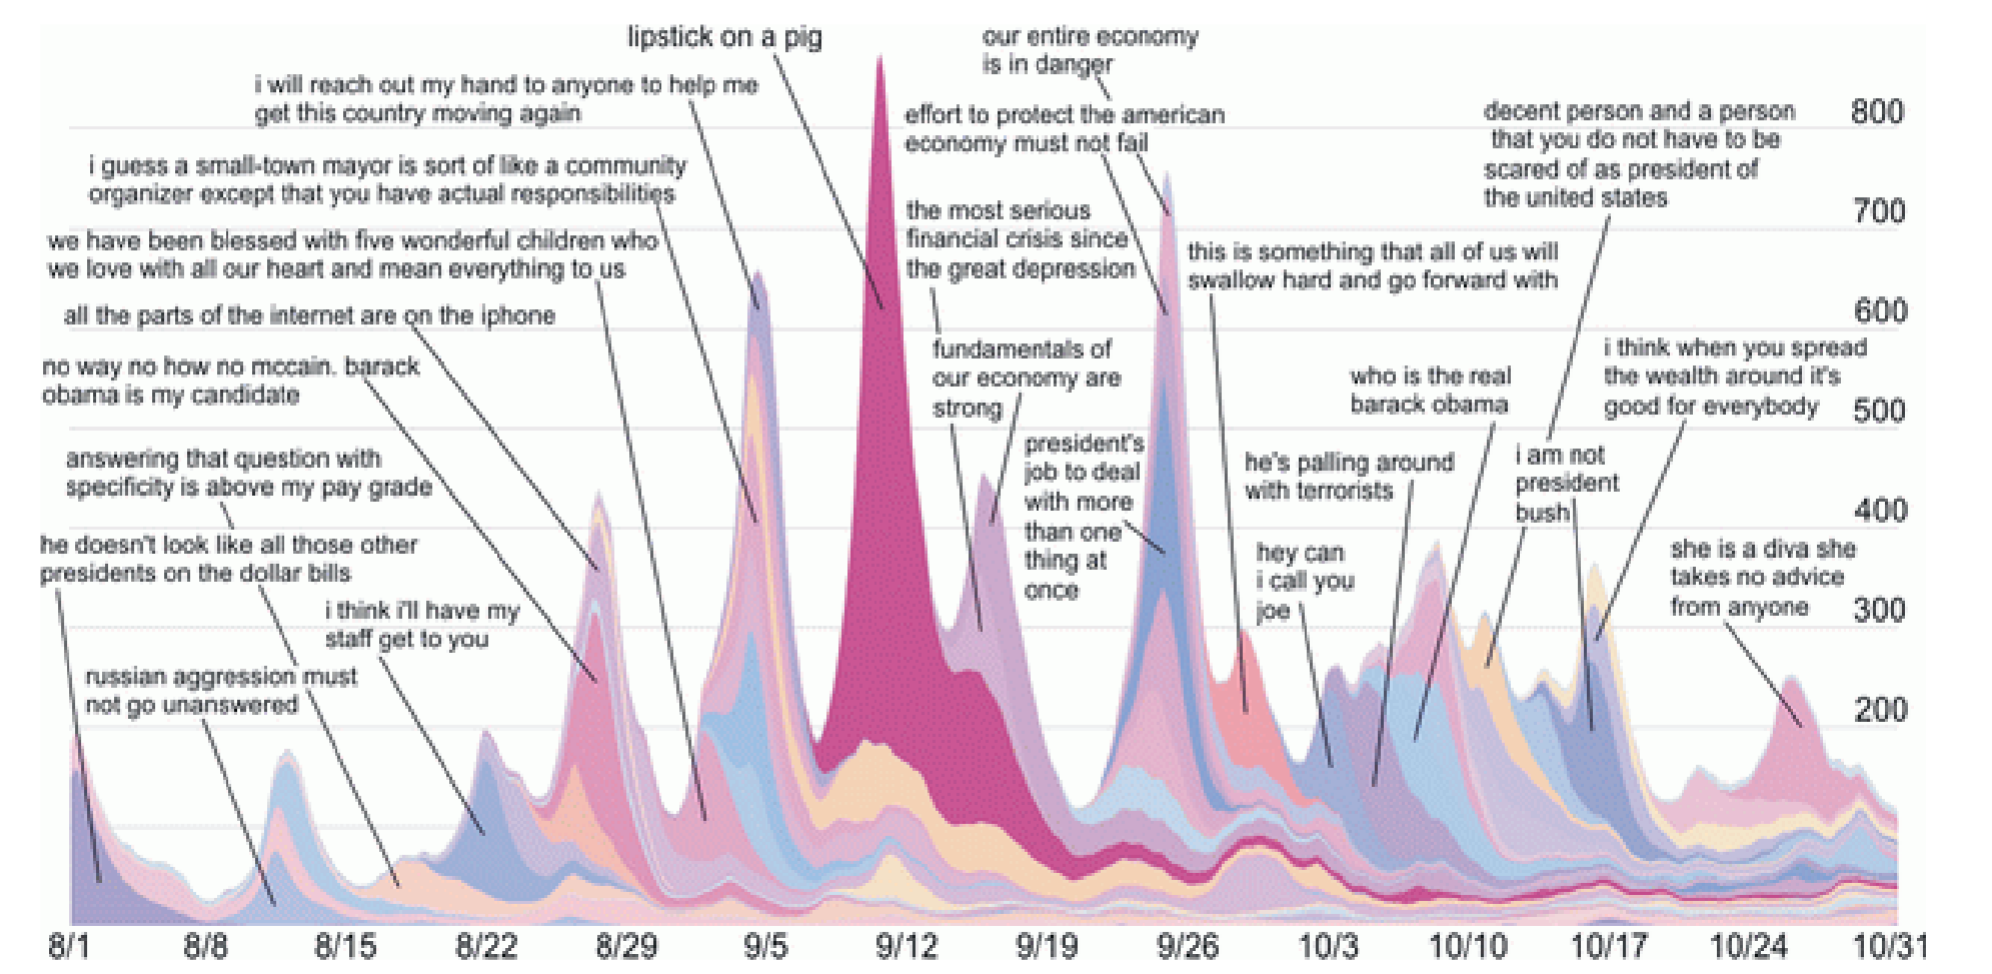
\includegraphics[width=\textwidth]{5.png}

what is it about "lipstick on a pig" that makes it go viral?
it is novel, it is surprising, it is interesting, it is complex, it is emotional
it is a story, it is a narrative, it is a meme.


\subsection{E.g. 3: Community detection}
\begin{itemize}
    \item Why detect communities?
    \item Simplified network structure and “big picture”
    \item Explain actions and positions
    \item Better predictions
    \item What defines a community?
    \item Interaction
    \item Profile
    \item Dynamics
    \item ...
\end{itemize}

\section{Social Network Analysis:
Preliminaries}
\subsection{What are networks?}
\begin{note}
    Networks are sets of nodes
    connected by edges.
\end{note}
“Network” = “Graph”

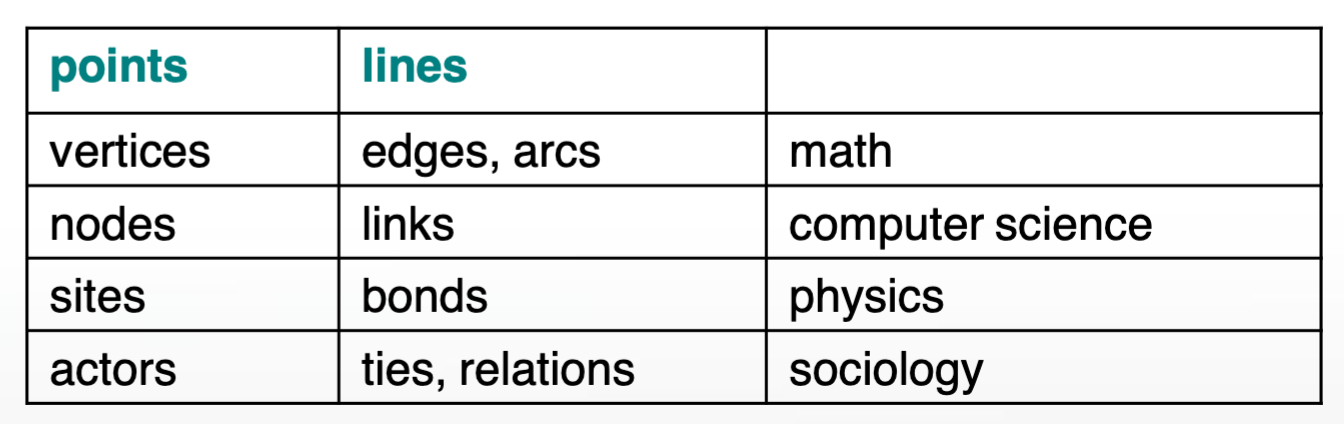
\includegraphics[width=\textwidth]{6.png}
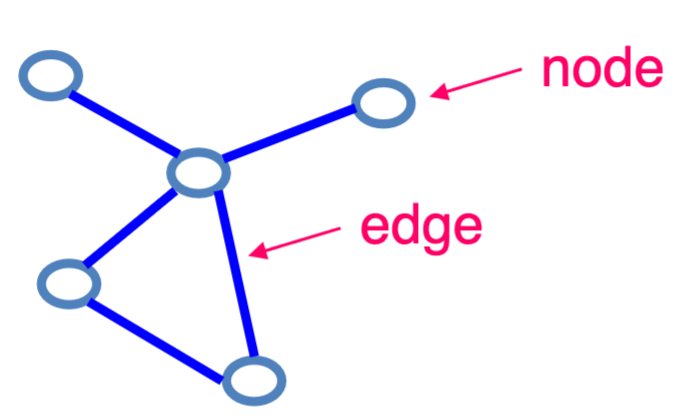
\includegraphics[width=\textwidth/2]{7.png}

\subsection{Network elements: edges}
Directed (also called arcs, links): A->B

Undirected: A<->B or A - B

Undirected is a subset of directed such that all undirected links have directed links

\subsection{Edge attributes}
Examples

\begin{itemize}
    \item weight (e.g. frequency of communication)
    \item ranking (best friend, second best friend...)
    \item type (friend, relative, co-worker)
    \item properties depending on the structure of the rest
    of the graph: e.g. betweenness
\end{itemize}

\subsection{Directed networks}
Girls’ school dormitory dining-table partners, 1st and 2nd choices
(Moreno, The sociometry reader, 1960)

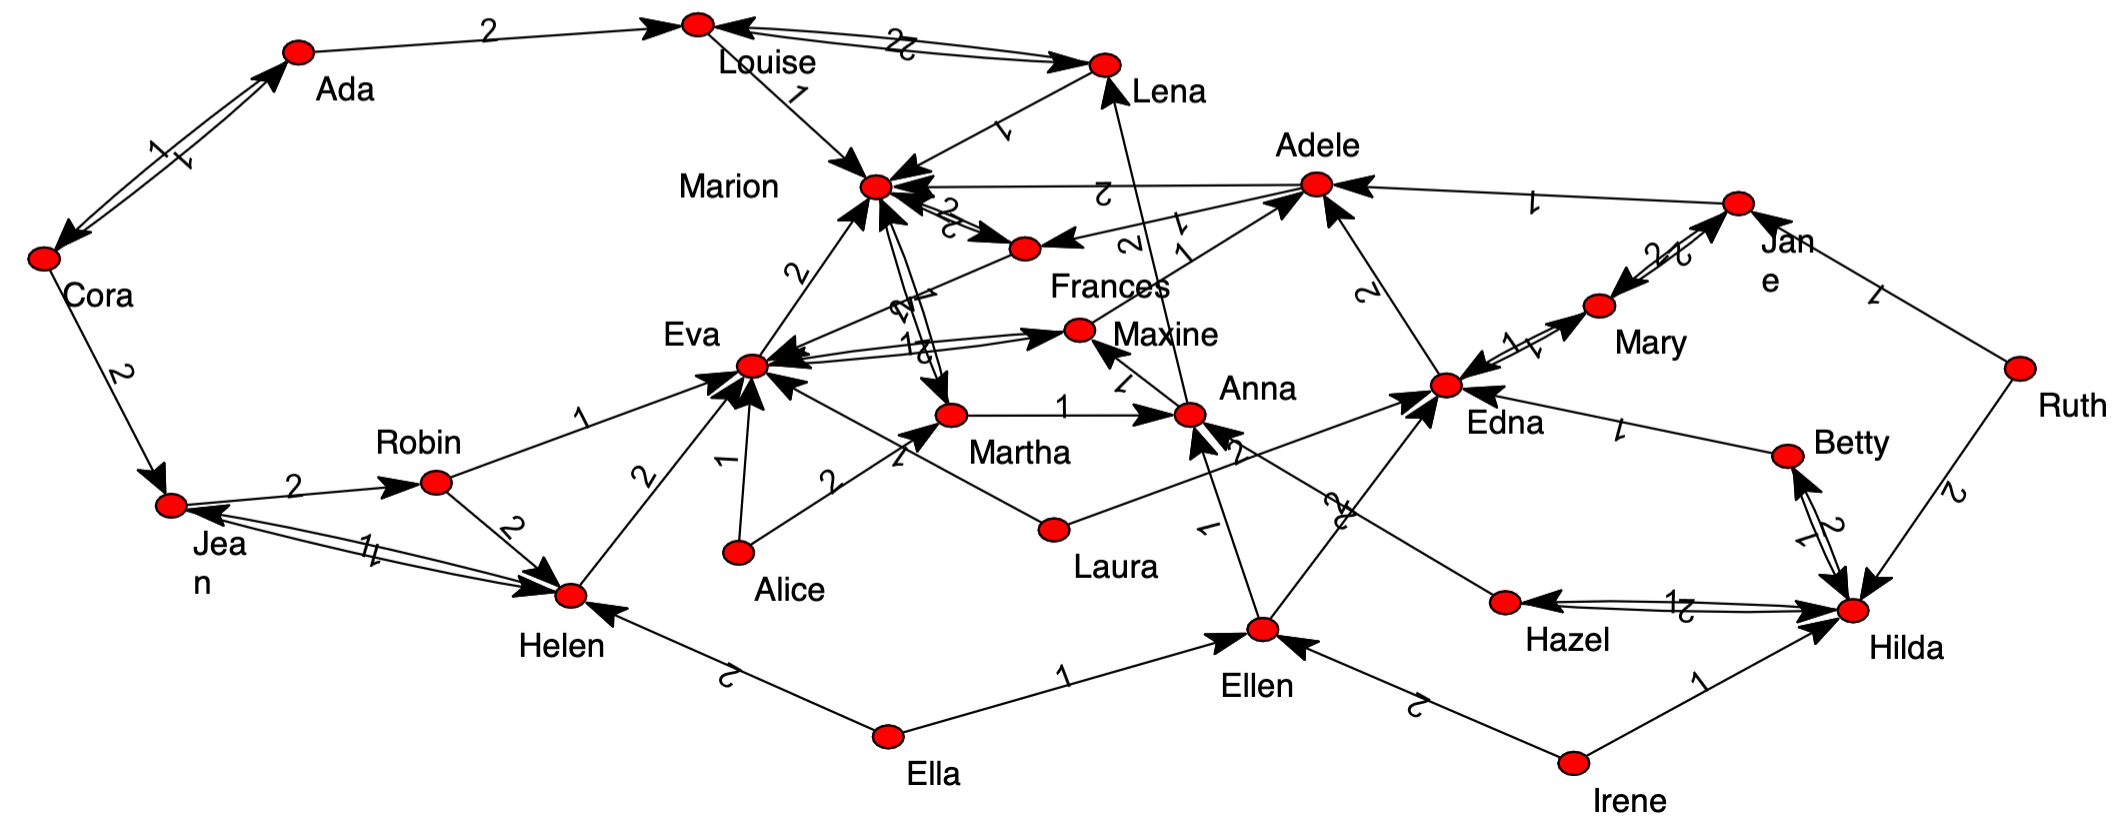
\includegraphics[width=\textwidth/2]{8.png}

\subsection{Document
Elements
In Twitter}
\begin{itemize}
    \item User
    \item Mention
    \item Hashtag
    \item Hyperlink
\end{itemize}

\section{Data representation}
\begin{enumerate}
    \item Adjacency matrix
    \item Edge list
    \item Adjacency list
\end{enumerate}

\subsection{(1) Adjacency matrices}
Representing edges (who is adjacent to whom) as a matrix

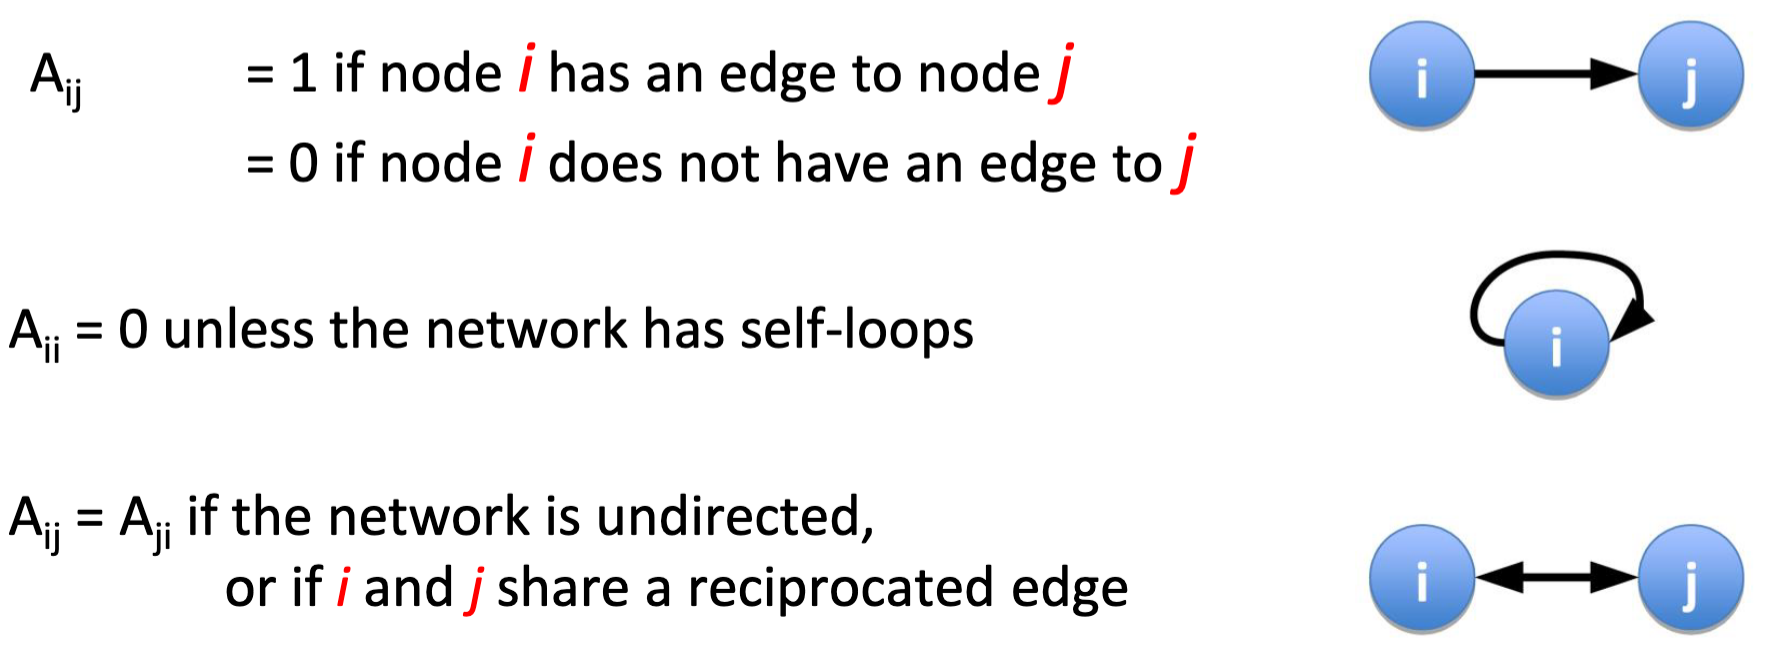
\includegraphics[width=\textwidth/2]{9.png}

\subsection{(1) Adjacency matrices example}
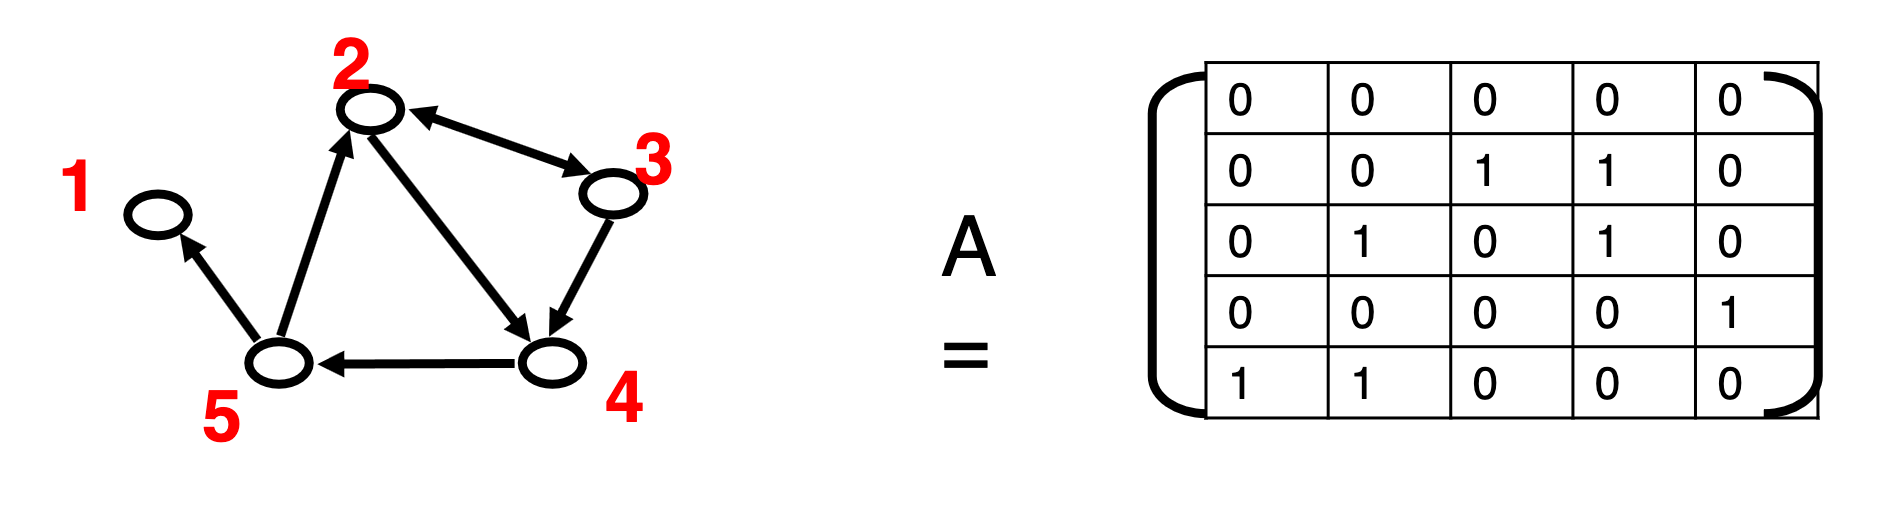
\includegraphics[width=\textwidth/2]{10.png}

\subsection{(2) Edge list}
\begin{itemize}
    \item 2, 3
    \item 2, 4
    \item 3, 2
    \item 3, 4
    \item 4, 5
    \item 5, 2
    \item 5, 1
\end{itemize}

\subsection{(3) Adjacency lists}
are easier to work with if
network is
• large
• sparse

quickly retrieve all neighbors
for a node

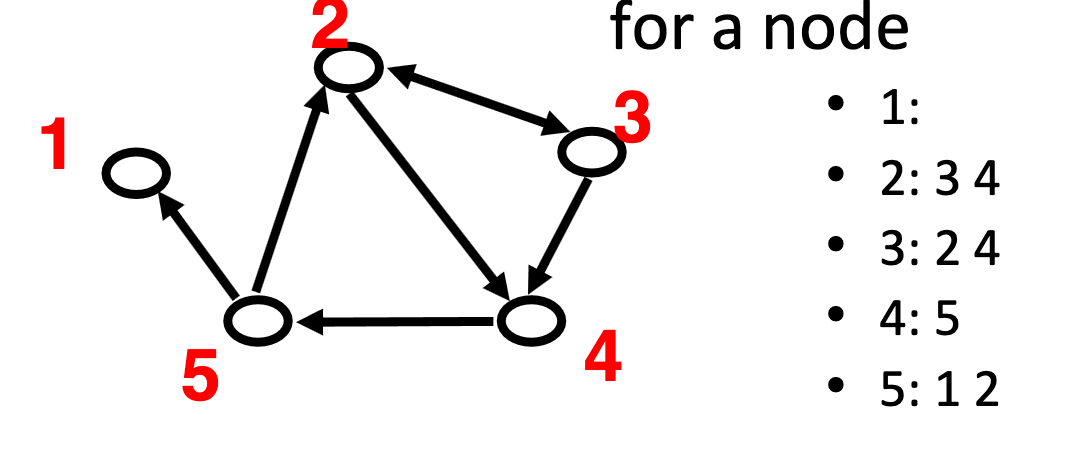
\includegraphics[width=\textwidth/2]{11.png}

stored as a key (dictionary) instead of a list. 
use a sparse matrix in python to store this.

\section{Computing metrics}
\begin{enumerate}
    \item Path and distance
    \item In/Out degree
    \item Centrality
\end{enumerate}

\subsection{Distances in a Network}
\begin{itemize}
    \item Path: a walk (i1,i2,... ik) with each node ij distinct
    \item Cycle: a walk where i1 = ik
    \item Geodesic: a shortest path between two nodes
\end{itemize}

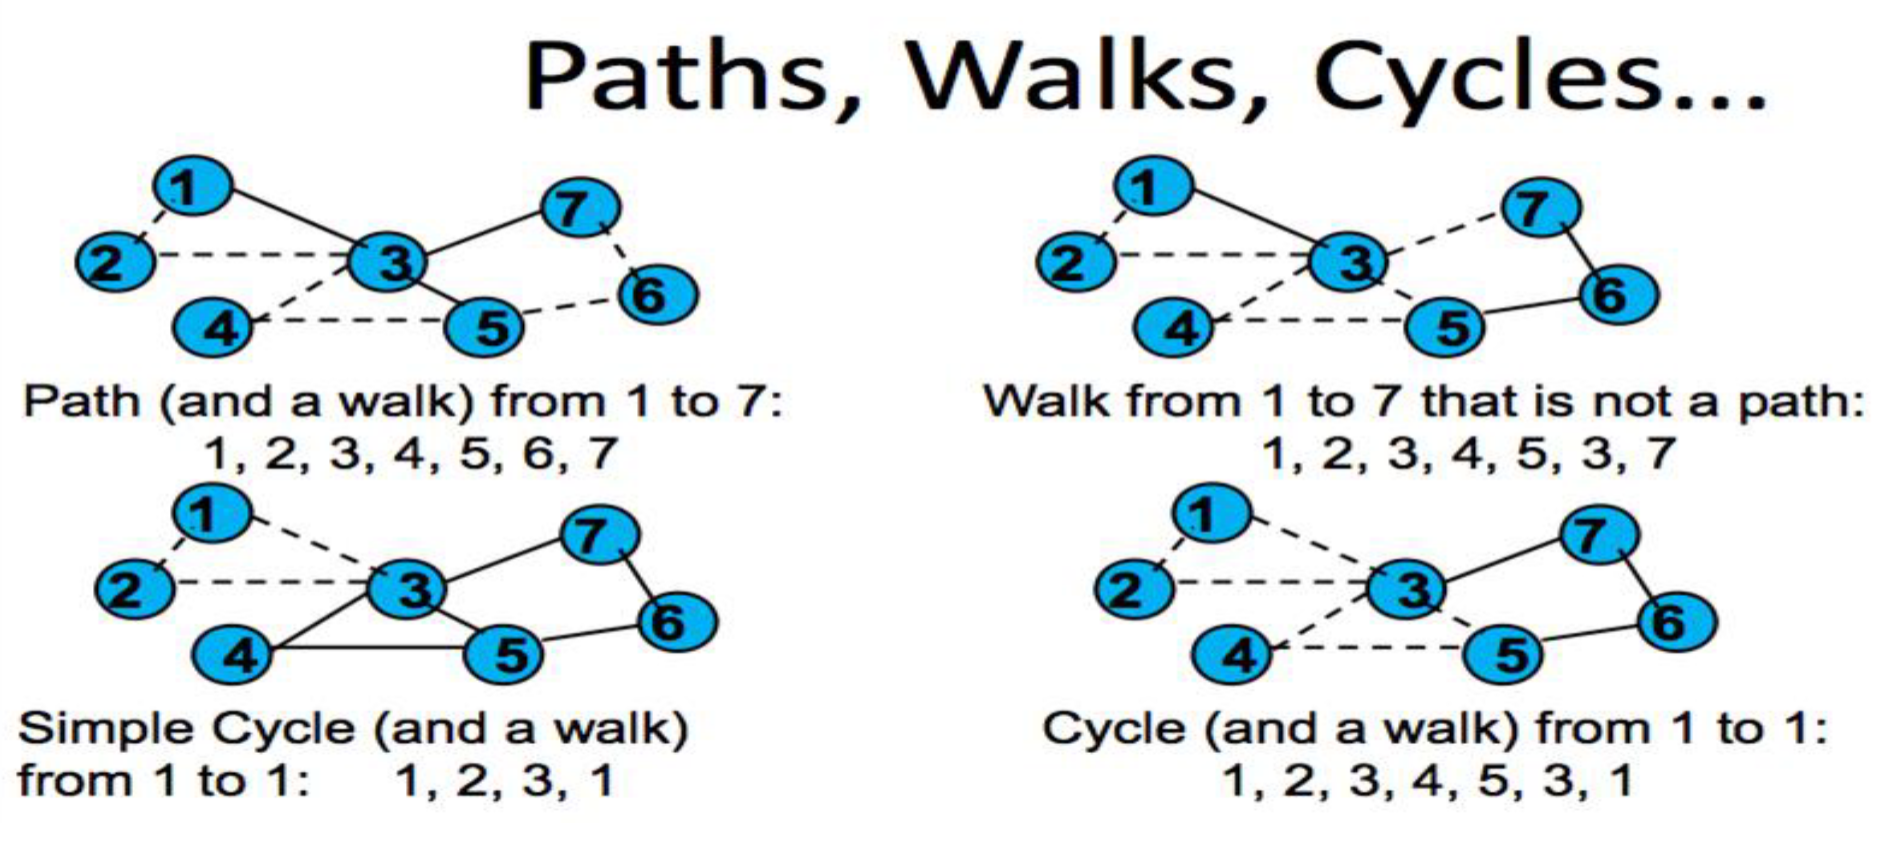
\includegraphics[width=\textwidth/2]{12.png}

\section{Who is the Center of a network?}
\subsection{Local view of the Social Network}
\begin{note}
    One centrality definition:
Nodes with more friends are more central.
\end{note}
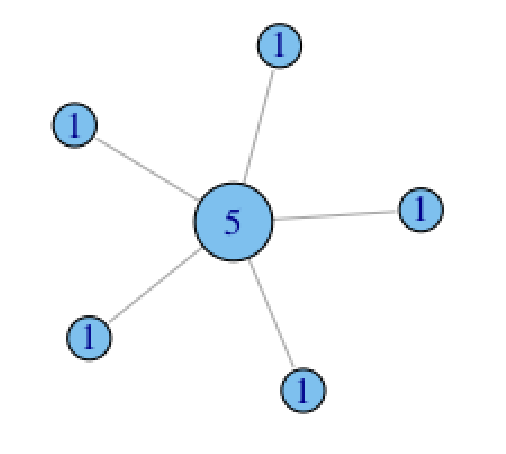
\includegraphics[width=\textwidth/5]{13.png}

Assumption: the connections that your friend has don't matter, it is what they
can do directly that does (e.g. go have a beer with you, help you build a
deck...)

\subsection{Indegree and Outdegree}
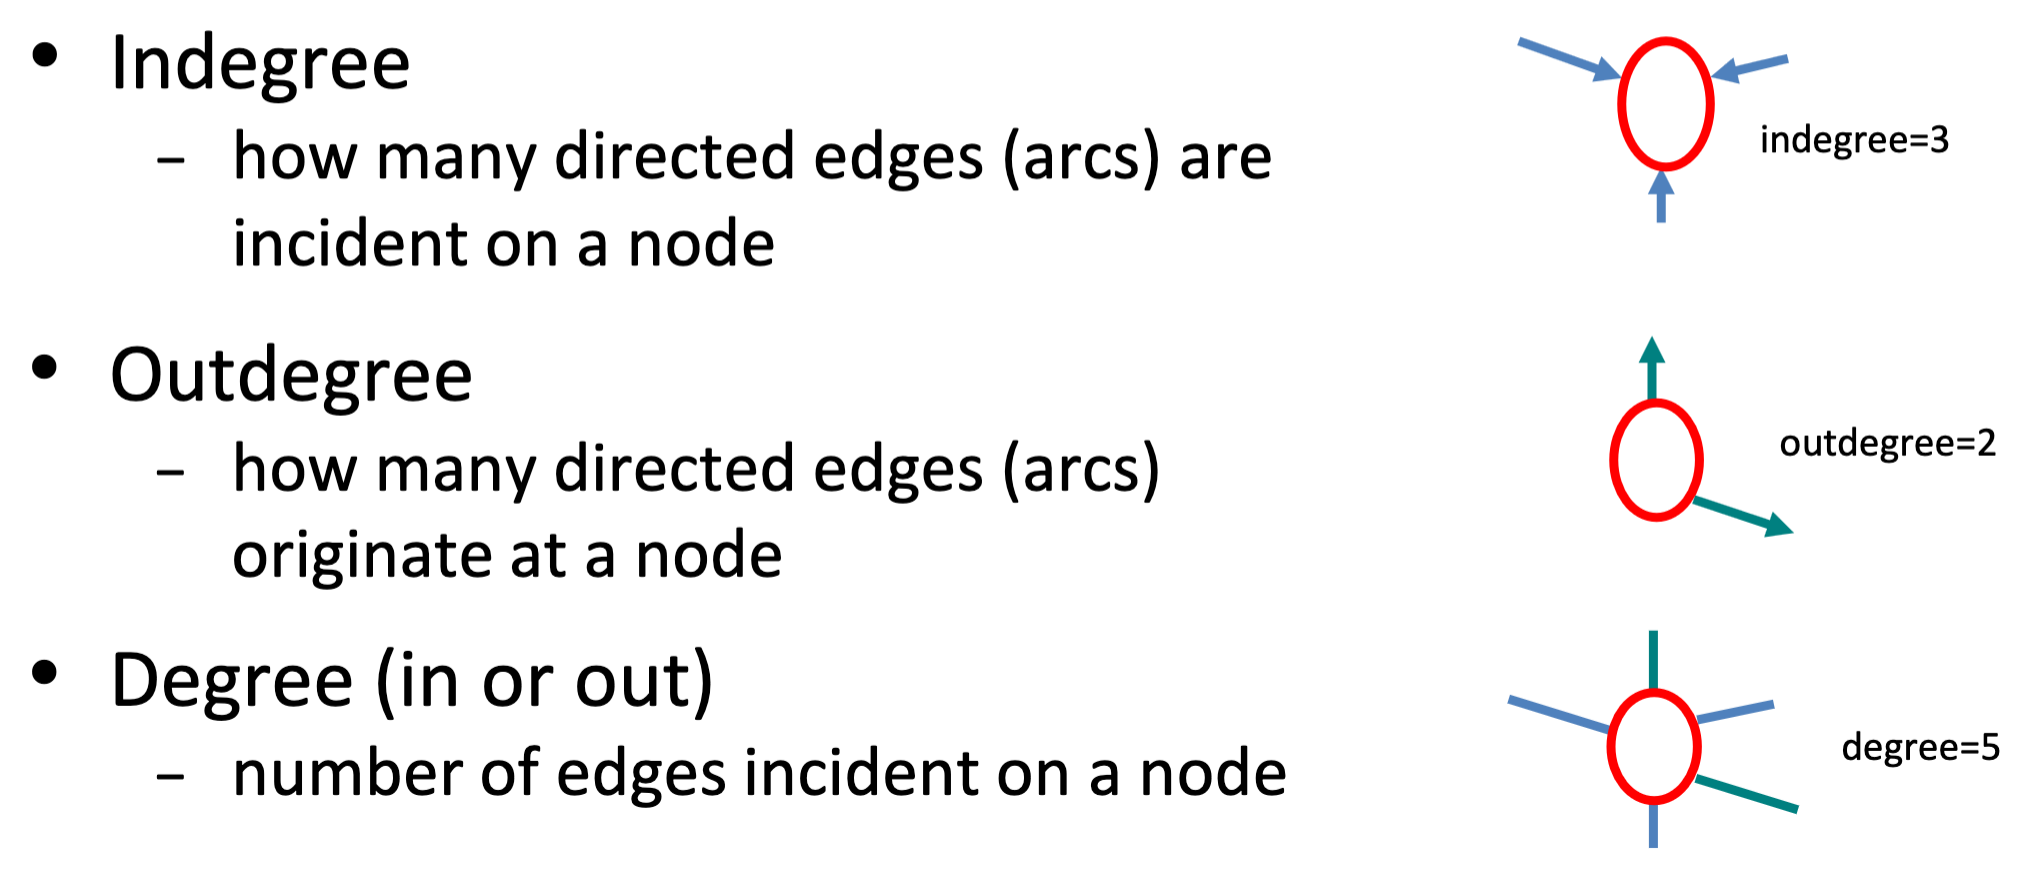
\includegraphics[width=\textwidth/2]{14.png}

\subsection{Node degree from matrix values}
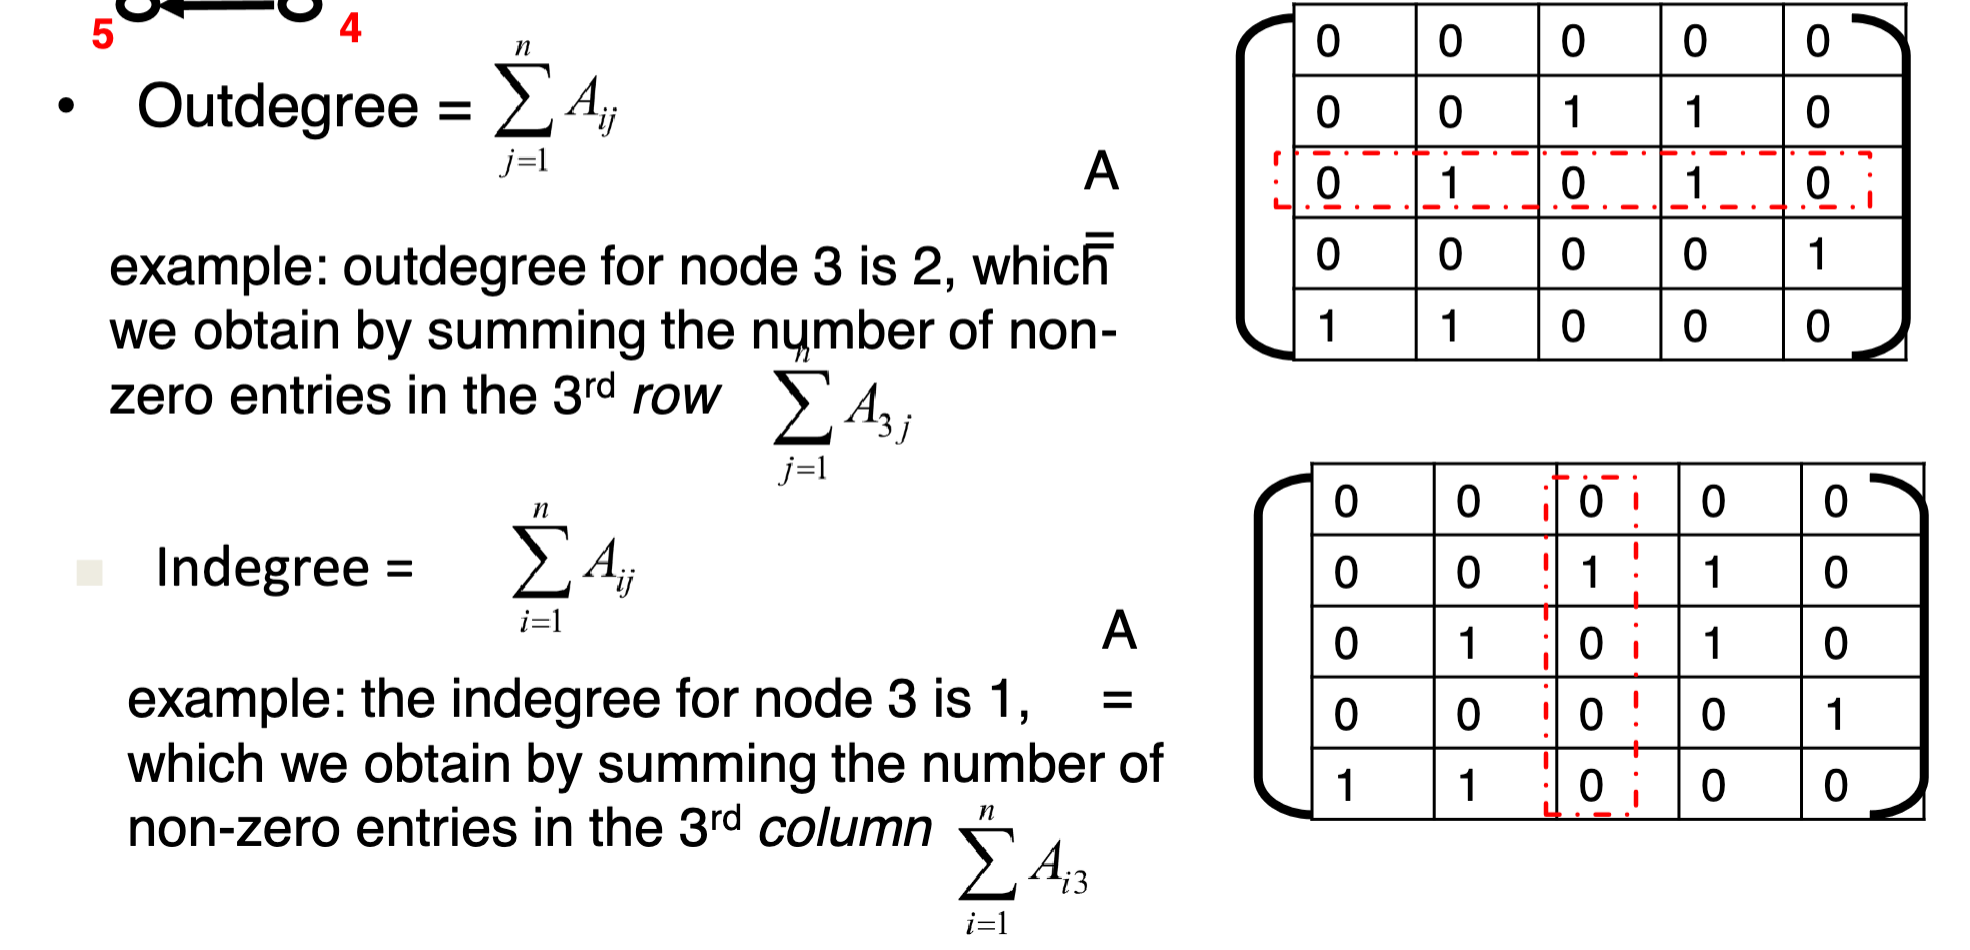
\includegraphics[width=\textwidth/2]{15.png}


\end{document}